% =============================================================================
%  SANEN KINSEN HIROKU — Three Monkeys Gold Spring Secret Record
%  English Translation
%
%  Original: 牛田権三郎 (Ushida Gonzaburō)
%  Revised:  鳴川猛之助 (Narukawa Takenosuke)
%  Manuscript source: Kyoto University Main Library, Tanimura Collection
%  Record ID: RB00012360
%  License: Free with Attribution (所蔵表示)
%
%  Compiled with XeLaTeX
% =============================================================================

\documentclass[11pt, openany]{book}

% --- Page geometry ---
\usepackage[
  papersize={6in,9in},
  margin=0.75in,
  inner=0.85in,
  outer=0.65in,
  top=0.8in,
  bottom=0.8in
]{geometry}

% --- Fonts (XeLaTeX) ---
\usepackage{fontspec}
\setmainfont{Noto Serif}[
  BoldFont={Noto Serif Bold},
  ItalicFont={Noto Serif Italic},
  BoldItalicFont={Noto Serif Bold Italic},
]
\newfontfamily\japanesefont{Noto Serif JP}
\newcommand{\jp}[1]{{\japanesefont #1}}

% --- Packages ---
\usepackage{graphicx}
\usepackage{xcolor}
\usepackage{titlesec}
\usepackage{fancyhdr}
\usepackage{enumitem}
\usepackage{booktabs}
\usepackage{microtype}
\usepackage{hyperref}
\usepackage{float}
\usepackage{setspace}
\usepackage{lettrine}
\usepackage{parskip}

% --- Colors ---
\definecolor{chaptercolor}{HTML}{8B0000}
\definecolor{sectioncolor}{HTML}{333333}
\definecolor{notecolor}{HTML}{555555}

% --- Chapter and section styling ---
\titleformat{\chapter}[display]
  {\normalfont\Large\bfseries\color{chaptercolor}}
  {\chaptertitlename\ \thechapter}{12pt}{\LARGE}
\titlespacing*{\chapter}{0pt}{-20pt}{20pt}

\titleformat{\section}
  {\normalfont\large\bfseries\color{sectioncolor}}
  {\thesection}{1em}{}

\titleformat{\subsection}
  {\normalfont\normalsize\bfseries\itshape\color{sectioncolor}}
  {\thesubsection}{1em}{}

% --- Headers and footers ---
\pagestyle{fancy}
\fancyhf{}
\fancyhead[LE]{\small\itshape Sanen Kinsen Hiroku}
\fancyhead[RO]{\small\itshape\leftmark}
\fancyfoot[CE,CO]{\small\thepage}
\renewcommand{\headrulewidth}{0.4pt}

% --- Footnote styling ---
\renewcommand{\footnotesize}{\small}

% --- Translator's note command ---
\newcommand{\tn}[1]{\footnote{\textit{Translator's note:} #1}}

% --- Japanese term with gloss ---
\newcommand{\jt}[2]{\jp{#1} (\textit{#2})}

% --- Epigraph-style block for maxims ---
\newenvironment{maxim}{%
  \begin{quote}\itshape
}{%
  \end{quote}
}

% --- Suppress chapter number in headers ---
\renewcommand{\chaptermark}[1]{\markboth{#1}{}}

% --- Hyperref setup ---
\hypersetup{
  colorlinks=true,
  linkcolor=chaptercolor,
  urlcolor=blue!60!black,
  pdftitle={Sanen Kinsen Hiroku: Three Monkeys Gold Spring Secret Record},
  pdfauthor={Ushida Gonzaburō; trans. Claude},
}

% =============================================================================
\begin{document}

% --- Half-title page ---
\thispagestyle{empty}
\begin{center}
\vspace*{2.5in}
{\Large\itshape Sanen Kinsen Hiroku}\\[0.5em]
{\large Three Monkeys Gold Spring Secret Record}
\vfill
\end{center}
\newpage
\thispagestyle{empty}
\mbox{}
\newpage

% --- Full title page ---
\thispagestyle{empty}
\begin{center}
\vspace*{1in}

{\huge\bfseries\color{chaptercolor} \jp{三猿金泉秘録}}\\[1em]
{\LARGE\bfseries Sanen Kinsen Hiroku}\\[0.7em]
{\Large\itshape Three Monkeys Gold Spring\\Secret Record}\\[2em]

\rule{3in}{0.5pt}\\[1.5em]

{\large\itshape A Secret Treatise on the Art of\\Rice Market Speculation}\\[0.5em]
{\normalsize from the Edo Period of Japan}\\[2.5em]

{\normalsize Written by}\\[0.3em]
{\large \jp{牛田権三郎}}\\
{\normalsize Ushida Gonzabur\=o}\\[1.5em]

{\normalsize Revised and Corrected by}\\[0.3em]
{\large \jp{鳴川猛之助}}\\
{\normalsize Narukawa Takenosuke}\\[2em]

\rule{3in}{0.5pt}\\[1.5em]

{\normalsize English Translation}\\[3em]

\end{center}
\vfill
\newpage

% --- Copyright / attribution page ---
\thispagestyle{empty}
\vspace*{\fill}
\begin{small}
\noindent\textbf{Source Manuscript}\\[0.3em]
\noindent\jp{校正三猿金泉秘録} (\textit{K\=osei Sanen Kinsen Hiroku})\\
Record ID: RB00012360\\
Tanimura Collection (\jp{谷村文庫})\\
Main Library, Kyoto University (\jp{京都大学附属図書館})\\[0.5em]
Manuscript note: Kaei 4 (1851), copy of \jp{好問亭蔵版本}\\[1em]

\noindent\textbf{Digital Images}\\[0.3em]
\noindent Kyoto University Rare Materials Digital Archive\\
\url{https://rmda.kulib.kyoto-u.ac.jp/item/rb00012360}\\[0.5em]
Free License with Attribution (\jp{二次利用自由（所蔵表示）})\\
Reuse policy: \url{https://rmda.kulib.kyoto-u.ac.jp/reuse}\\[1em]

\noindent\textbf{Attribution}\\[0.3em]
\noindent All manuscript images courtesy of the Main Library, Kyoto University.\\
\jp{所蔵：京都大学附属図書館}\\[1em]

\noindent\textbf{About This Translation}\\[0.3em]
\noindent This is a working English translation of an Edo-period manuscript on
rice market speculation, produced with AI assistance. The original text is
written in classical Japanese (\textit{kobun}) with \textit{kanbun kundoku}
reading marks. Due to the difficulty of the source material---hand-written
cursive script on aged paper---some readings are approximate. Specialist
terms are glossed in footnotes.\\[1em]
\end{small}
\newpage

% =============================================================================
% TABLE OF CONTENTS
% =============================================================================
\thispagestyle{empty}
\tableofcontents
\newpage

% =============================================================================
% TRANSLATOR'S INTRODUCTION
% =============================================================================
\chapter*{Translator's Introduction}
\addcontentsline{toc}{chapter}{Translator's Introduction}
\markboth{Translator's Introduction}{}

The \textit{Sanen Kinsen Hiroku} (\jp{三猿金泉秘録}), or ``Three Monkeys
Gold Spring Secret Record,'' is one of the most celebrated texts in the history
of Japanese market speculation. Attributed to Ushida Gonzabur\=o
(\jp{牛田権三郎}), it circulated as a secret family manuscript before being
revised and published by Narukawa Takenosuke (\jp{鳴川猛之助}) in the
mid-nineteenth century.\tn{The catalog entry for the Kyoto University
manuscript notes ``Kaei 4'' (1851) and identifies it as a copy of the
\jp{好問亭蔵版本} (K\=omond\=o edition). The text itself references the
Tenmei era (1781--1789) extensively.}

The title alludes to the proverb of the three monkeys---``see no evil, hear
no evil, speak no evil'' (\jp{見ざる、聞かざる、言わざる})---here reinterpreted
as a warning to the trader: do not be swayed by what you \textit{see} others
doing, what you \textit{hear} as rumor, or what you \textit{say} in haste.
Instead, observe the deeper patterns.

\section*{The Edo Rice Market}

During the Tokugawa period (1603--1868), rice was not merely a commodity but
the basis of the entire economy. Samurai stipends were paid in rice, domain
revenues were calculated in rice, and the great rice exchanges---above all
the D\=ojima Rice Exchange (\jp{堂島米会所}) in Osaka---functioned as
sophisticated futures markets where ``book rice'' (\jp{帳合米}) was traded
as forward contracts.\tn{The D\=ojima exchange, established in 1697, is often
cited as the world's first organized futures market. The trading methods
described in this text would have been applied there.}

The text belongs to a genre known as \jp{相場秘伝書} (\textit{s\=oba
hidensho})---``secret market transmission texts''---which circulated among
trading houses as closely guarded family knowledge. Many such texts were
attributed to the legendary Honma Munehisa of Sakata, though the present
text names Ushida Gonzabur\=o as its author.

\section*{Structure of the Text}

The manuscript covers several interconnected domains:

\begin{enumerate}[leftmargin=2em]
\item \textbf{Cosmological framework}: The market is understood through
  Yin-Yang (\jp{陰陽}) theory and the Neo-Confucian concept of the Supreme
  Ultimate (\jp{太極}).
\item \textbf{Cyclical analysis}: Multi-year cycles of favorable
  (\jp{順来}) and adverse (\jp{逢来}) market conditions, correlated with
  the sixty-year sexagenary calendar.
\item \textbf{Weather forecasting}: Detailed correlations between the
  sexagenary cycle and weather patterns---storms, floods, frost, plum
  rains---as predictors of harvest outcomes.
\item \textbf{The Middle Star system}: A mean-reversion framework using a
  long-term average price level (the \jp{中星}, ``middle star'') as the
  reference point for all trading decisions.
\item \textbf{Position management}: Systematic methods of staged entry and
  exit, with detailed numerical examples showing how to compound returns.
\item \textbf{Trading psychology}: Teachings on patience, discipline, and
  the danger of following the crowd.
\end{enumerate}

\noindent What follows is the complete text in translation, organized into
chapters for clarity.

\vspace{1em}
\begin{flushright}
\textit{---The Translator}
\end{flushright}

% =============================================================================
% CHAPTER 1: PREFACE
% =============================================================================
\chapter{Preface: The Cosmology of the Market}

\begin{center}
\jp{三猿金泉録序}\\
\textit{Preface to the Three Monkeys Gold Spring Record}
\end{center}

\vspace{1em}

\lettrine[lines=2]{T}{he Supreme Ultimate}\tn{\jp{太極} (\textit{taikyoku}).
The foundational concept in Neo-Confucian cosmology, representing the
undifferentiated unity from which Yin and Yang emerge. The opening
deliberately echoes Zhou Dunyi's \textit{Taijitu shuo} (Explanation of the
Diagram of the Supreme Ultimate, 1070s), grounding market theory in the
highest philosophical authority.}
moves and gives birth to Yang; when still, it gives birth to Yin.
The principle of one stillness and one movement---Heaven and Earth rise and
fall according to this logic. Movement reaches its extreme and becomes
stillness; stillness reaches its extreme and becomes movement again.
Movement and stillness are the root of one another.

This is the principle by which strong qi\tn{\jp{強気} (\textit{tsuyoki}),
literally ``strong spirit.'' In market contexts, this corresponds to bullish
sentiment or upward momentum. Its opposite, \jp{弱気} (\textit{yowaki}),
``weak spirit,'' corresponds to bearish sentiment.} and weak qi alternate.

When this principle is applied to all things, there is nothing it does not
encompass. When applied to rice, the qi of people---whether strong or
weak---is contained within this principle. Those who combine this
understanding with close observation of the market will find it reasonable.
In years of good harvests and times of fine weather, one should compare and
examine the rice markets.

This is the principle that transcends mere natural disposition.

% =============================================================================
% CHAPTER 2: FAVORABLE AND ADVERSE CONDITIONS
% =============================================================================
\chapter{The Way of Favorable and Adverse Conditions}

\begin{center}
\jp{順来・逢来} --- \textit{Junrai and Airai}
\end{center}

\vspace{1em}

The market moves in great cycles of favorable conditions (\jt{順来}{junrai})
and adverse conditions (\jt{逢来}{airai}). Within a period of roughly
twelve to thirteen years, favorable conditions persist for approximately ten
years, and adverse conditions for three.\tn{This roughly 10:3 ratio of
bull-to-bear years is a recurring theme. While the specific ratio is
debatable, the underlying insight---that markets spend more time rising than
falling, but that the falls are sharper---remains relevant.}

\section{Favorable-Condition Years}

During favorable years, rice is generally at high levels. When old rice
(\jt{古米}{komai})\tn{``Old rice'' refers to rice from previous harvests,
as opposed to \jp{新米} (\textit{shinmai}), newly harvested rice. Old rice
was traded as a distinct commodity with its own price dynamics.} is in a year
of abundance, it will be cheap:

\begin{maxim}
Buy in the fourth month. By mid-sixth month, prices will be high---this is
where one sells. In autumn, buy again around the seventh month. Toward
year-end, the price of old rice will rise, and one should sell again.
\end{maxim}

This is the fundamental seasonal pattern of favorable years.

\section{Adverse-Condition Years}

In adverse years, the cheap period for old rice falls around the fourth
through sixth months. In autumn, one should buy, and by year-end the rice
price climbs. But the overall trajectory is downward---the trader must be
more cautious, take smaller positions, and be quicker to exit.

\section{Songs of the Seasons}

\begin{maxim}
In a year of favorable conditions, the autumn harvest is plentiful;\\
the highs and lows can be estimated across four seasons.\\[0.5em]
In spring, from around the fourth month onward,\\
buy at the fifth-month level;\\
by the end of the year, the high price will come.
\end{maxim}

\section{Monthly Sentiment}

In favorable-condition periods, the rice market's sentiment
(\jt{人気}{jinki})\tn{Literally ``people-qi''---the collective mood or
energy of market participants. A remarkably modern concept of market
sentiment.} for each month can be read directly. The fifth-month and
year-end levels become the reference points.

In a year of great flood (\jt{大水}{ōmizu}), the rice market reacts through
the twelfth month. Monthly sentiment varies, and autumn rice trades at its
own independent level.

% =============================================================================
% CHAPTER 3: THE FIFTEEN ARTICLES
% =============================================================================
\chapter{The Fifteen Articles of Trading}

\begin{center}
\jp{十五ヶ条}\\
\textit{Jūgo Kajō}
\end{center}

\vspace{1em}

Among the provisions for trading, those who deal in large quantities and
those with small capital must both observe the following.

\section{On Market Sentiment}

Within the market, one must read the sentiment of the crowd---whether people
are inclined to buy or sell---and not act rashly.

\begin{maxim}
The large trader may think that because he has capital, he can afford to hold
a losing position. This is a grave error.
\end{maxim}

Even with great capital, if one buys recklessly and the market moves against
him, the losses compound. Conversely, a trader of modest means who reads the
market well and trades with discipline can accumulate wealth steadily.

\section{On the Judgment of Buying and Selling}

The decision to buy or sell should not be made lightly. One should observe
for several days:

\begin{maxim}
When the rice price has been falling and reaches a point where it no longer
declines despite bad news---this is the moment to buy.\\[0.5em]
When rice has been rising and ceases to advance despite favorable
reports---this is the moment to sell.
\end{maxim}

\section{On the Danger of Following the Crowd}

Do not follow the crowd blindly. When all are buying, consider selling; when
all are selling, consider buying. The profit lies in going against common
sentiment, yet one must have sound reason for doing so.\tn{This contrarian
principle is perhaps the most famous teaching of the Edo-period market texts.
It anticipates modern behavioral finance concepts like ``buy when there is
blood in the streets'' (attributed to Baron Rothschild) by roughly a century.}

% =============================================================================
% CHAPTER 4: THE METHOD OF STAGED ENTRY
% =============================================================================
\chapter{The Method of Staged Entry}

\begin{center}
\jp{萬光商内之圖}\\
\textit{Bankō Shōnai no Zu --- Diagram of Ten-Thousand-Light Trading}
\end{center}

\vspace{1em}

The secret of profitable trading lies not in any single transaction but in the
\textit{method} of building and unwinding positions through stages.

\section{The Tree Diagram}

\begin{figure}[H]
\centering
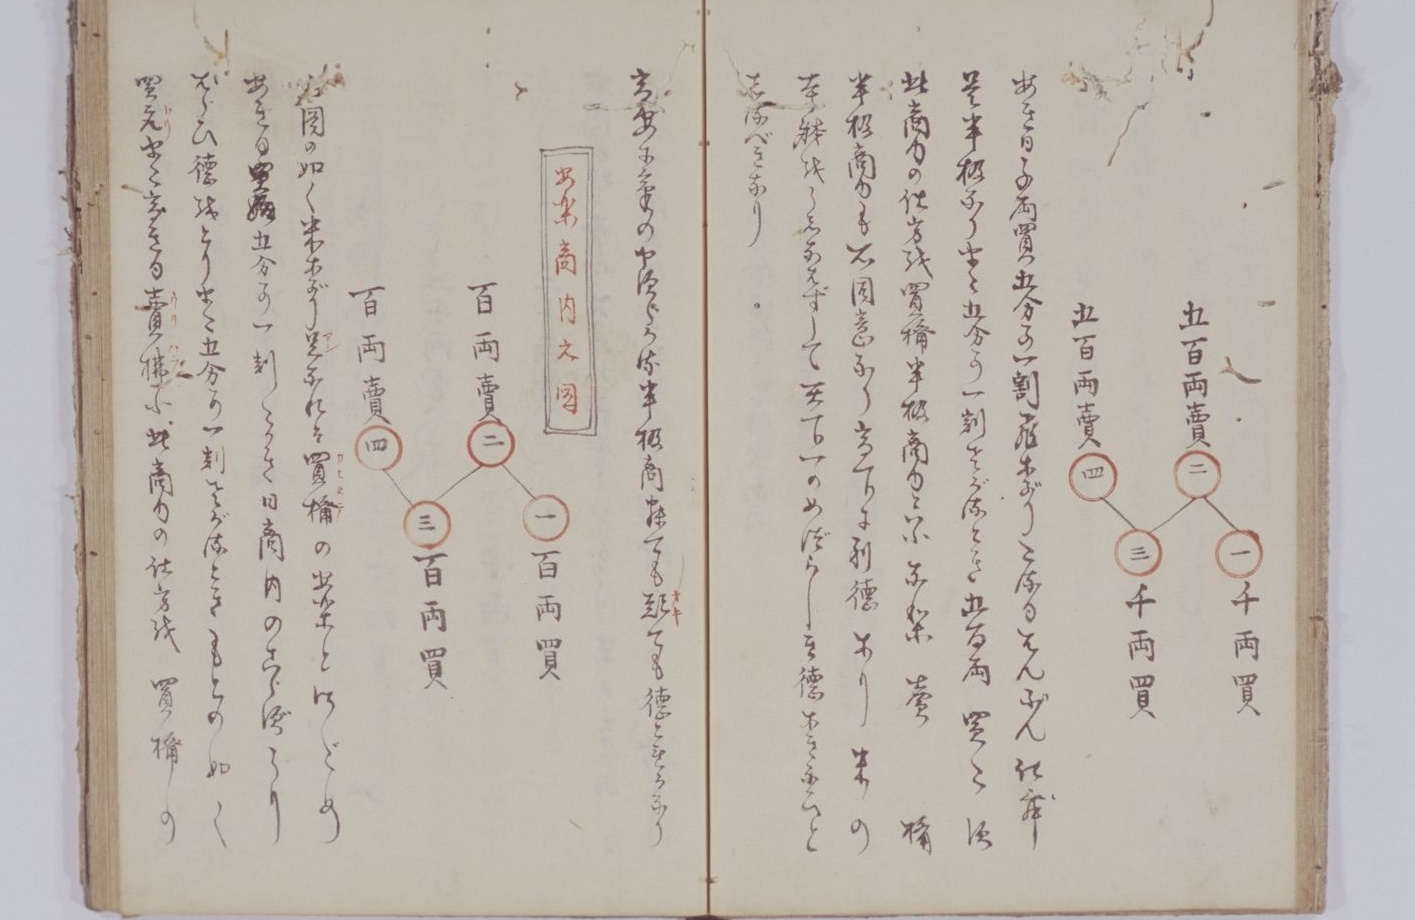
\includegraphics[width=\textwidth]{diagrams/fig1_tree_positions.jpg}
\caption{Position-scaling tree diagrams. Right: building from a 1,000-ryō
base purchase (\jp{千十両買}) through four stages to a 500-ryō sell position
(\jp{五百両買}). Left: the 100-ryō sell diagram (\jp{百両売}) with title
cartouche \jp{萬光商内之圖}.
\textit{Image: Kyoto University Main Library.}}
\label{fig:tree1}
\end{figure}

Starting from a base purchase, one builds the position through numbered
stages:

\begin{enumerate}[leftmargin=2em]
\item \textbf{Stage One} (\jp{壱}): A small, probing entry---the initial
  commitment of capital. This tests the market's direction.
\item \textbf{Stage Two} (\jp{弐}): When the direction is confirmed, a
  larger addition is made.
\item \textbf{Stage Three} (\jp{参}): Further addition as confidence grows.
\item \textbf{Stage Four} (\jp{四}): The position reaches its full size.
\end{enumerate}

The same principle applies in reverse when selling: one does not liquidate
the entire position at once but sells in stages, observing the market's
reaction at each step.

\section{Scaling to Larger Positions}

\begin{figure}[H]
\centering
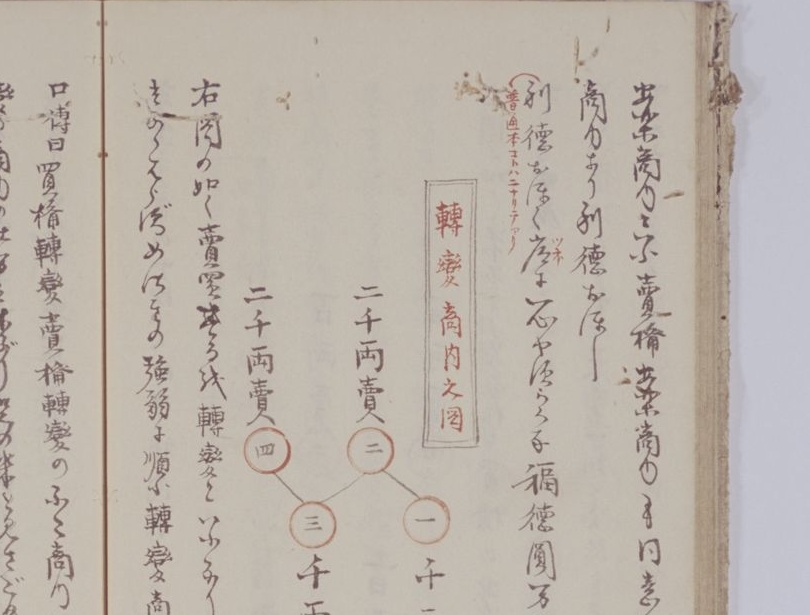
\includegraphics[width=0.8\textwidth]{diagrams/fig2_tree_scaling.jpg}
\caption{The scaling diagram for larger capital: \jp{転愛商内之圖}
(\textit{Diagram of Revolving Trading}). A 1,000-ryō buying position
(\jp{千両買}) builds through four stages to a 2,000-ryō selling position
(\jp{二千両売}). \textit{Image: Kyoto University Main Library.}}
\label{fig:tree2}
\end{figure}

When buying positions reach their target, one begins to build selling
positions simultaneously---this is called the ``turnover method''
(\jt{転換の法}{tenkan no hō}). For every 1,000 ryō in buying positions,
prepare to sell 2,000 ryō worth. The reasoning: as the market reaches its
peak, the momentum of the crowd drives prices beyond fair value. The
disciplined trader sells more than he bought, profiting from the overshoot.

\section{On Trading Psychology}

\begin{maxim}
When traders buy at low prices and see profits growing, they become greedy
and wish to hold longer. When they see losses, they become fearful and wish
to sell at once. Both impulses are the enemy of profit.\\[0.5em]
The disciplined trader sells when he wishes to hold, and holds when he
wishes to sell---going against his own emotions as well as those of the crowd.
\end{maxim}

This art was not to be shared lightly. It was passed down within the family
and among trusted associates only.

% =============================================================================
% CHAPTER 5: SIXTY-YEAR WEATHER CYCLE
% =============================================================================
\chapter{The Sixty-Year Cycle: Weather and Harvest Prediction}

\begin{center}
\jp{暴風 運気豊凶之録}\\
\textit{Record of Storms, Fortune-Qi, and Abundance or Famine}
\end{center}

\vspace{1em}

A twelve-year sub-cycle governs the alternation of fortune and misfortune in
harvests. Two hundred and thirty years of records were consulted, tracking
patterns of favorable weather, adverse conditions, and their correlation
with the sexagenary cycle.\tn{The sexagenary cycle (\jp{干支},
\textit{kanshi} or \textit{eto}) combines the ten Heavenly Stems and twelve
Earthly Branches to produce a sixty-year cycle. Each year has a unique
two-character designation (e.g., \jp{甲子}, \textit{kinoe-ne}). This
system was used across East Asia for calendrical and divinatory purposes.}

\section{Violent Storms}

In certain years of the cycle, violent storms and market surges are more
frequent:

\begin{quote}
\jp{甲子}, \jp{丁卯}, \jp{丁未}, \jp{甲戌}, \jp{甲申}, \jp{辛卯}, \jp{甲午}
\end{quote}

In these years, rice markets experience extreme volatility; prices may surge
two or three times within a single season.

\section{Floods}

Years containing \jp{己} (\textit{tsuchinoto}) in their stem are associated
with water disasters:

\begin{quote}
\jp{己巳}, \jp{己卯}, \jp{己丑}, \jp{己亥}, \jp{己酉}, \jp{己未}
\end{quote}

These bring three-year periods of disruption. Rice prices respond sharply.

\section{Frost and Cold}

Unusual cold damages crops and triggers three-year adverse periods. Rice
prices rise sharply in response.

\section{Bountiful Harvest Years}

Years of expected bountiful harvest (\jt{豊作}{hōsaku}) were tracked across
twenty-eight years of records and correlated with sexagenary years. In
autumn months, the yields were logged, producing a predictive framework
that held across the full sixty-year cycle.

\section{The Plum Rains}

The onset of the \textit{tsuyu} (\jp{梅雨}) rainy season follows an
approximately eight-year sub-cycle:

\begin{maxim}
Early plum rains generally indicate good harvests.\\
Late plum rains may indicate drought followed by flooding.
\end{maxim}

% =============================================================================
% CHAPTER 6: THE EIGHT POLES
% =============================================================================
\chapter{The Eight Poles and Celestial Signs}

\begin{center}
\jp{八極 三千目}\\
\textit{Hakkyoku Sanzenme --- Eight Poles, Three Thousand Points}
\end{center}

\vspace{1em}

The eight extremes of market behavior, observable across all conditions,
represent the outer boundaries of price movement. Beyond these poles, the
market must reverse.

\section{The General's Campaign}

\begin{maxim}
Just as a general must commit his forces decisively at the right moment, the
trader must commit capital when the signs align. Hesitation at the critical
moment means the opportunity passes.
\end{maxim}

The categories of market force are classified:

\begin{itemize}[leftmargin=2em]
\item \jt{陽}{Yō} --- Yang: the bullish, rising force
\item \jt{陰}{In} --- Yin: the bearish, falling force
\item \jt{太極}{Taikyoku} --- Supreme Ultimate: the equilibrium point
\item \jt{陰合}{Ingō} --- Yin convergence: multiple bearish factors aligning
\end{itemize}

\section{The Unanimity Signal}

When ten thousand people are all of one mind---all buying or all selling---the
reversal is near:

\begin{maxim}
A thousand people of the same opinion is a strong signal.\\
Ten thousand unanimous is an extreme.\\
At such moments, the solitary trader who goes against them has the advantage.
\end{maxim}

\section{Celestial Anomalies}

When extraordinary signs appear---unusual weather, disruptions to the normal
seasonal flow---the trader must first determine whether these are temporary
or lasting in their effect. The standard rice price across months, the
ordinary level (\jt{普通}{futsū}), is established over a year, and only
deviations from this level are traded.

% =============================================================================
% CHAPTER 7: THE FIVE VIRTUES
% =============================================================================
\chapter{The Five Virtues of the Trader}

The text organizes its deepest teachings around the Confucian virtues,
applying each to the art of trading.

\section{Benevolence (\jp{仁}, \textit{Jin})}

\begin{maxim}
Buy once, and it returns to its original level. Wait.
\end{maxim}

When one buys and the price immediately returns to the purchase level, one
must not panic and sell at cost. The market is testing the trader's resolve.
This is the test of benevolence---patience and compassion for one's own
position.

If after buying, the price falls and then recovers to near the purchase
price, this pattern---repeated over three years---teaches the trader to
endure. In each of those years, the rice that was bought at what seemed a
bad time eventually proved profitable for those who held.

\subsection{On Upper, Middle, and Lower Positions}

\begin{itemize}[leftmargin=2em]
\item \textbf{Upper level} (\jt{上位}{jōi}): rice has risen strongly and
  is at the top of its range. \textit{One should be selling, not buying.}
\item \textbf{Middle level} (\jt{中位}{chūi}): rice is at its ordinary
  seasonal level. \textit{Wait and observe.}
\item \textbf{Lower level} (\jt{下位}{gei}): rice has fallen to the bottom
  of its range. \textit{This is where buying begins.}
\end{itemize}

\begin{maxim}
When the price has been at a low level for three hundred days or more, and a
rise begins, and then the price returns and falls again to a new low---this
is the final bottom. Buy here.
\end{maxim}

\section{Wisdom (\jp{智}, \textit{Chi})}

Wisdom in trading has multiple aspects: knowing when to enter, knowing when
to exit, reading the mood of the market, understanding seasonal patterns,
and patience in waiting for the right moment.

The relationship between different regional markets---D\=ojima, Bakan, and
others---and how information flows between them creates timing advantages.
The trader who understands this flow profits from the gap.

\section{Courage (\jp{勇}, \textit{Yū})}

The courage to act when the signs align, even when the crowd moves in the
opposite direction. Courage without wisdom is recklessness; wisdom without
courage is paralysis.

\section{Discipline (\jp{節}, \textit{Setsu})}

Following the method even when emotions urge otherwise. The disciplined
trader who holds reserves of twenty tawara and trades with five will
survive all storms. He who trades with his entire fortune will eventually
be ruined.

% =============================================================================
% CHAPTER 8: THE THREE LEVELS AND THE MIDDLE STAR
% =============================================================================
\chapter{The Three Levels and the Middle Star}

\begin{center}
\jp{世の中 三段之圖}\\
\textit{Yo no Naka Sandan no Zu --- Diagram of the Three Levels of the World}
\end{center}

\vspace{1em}

This chapter contains the core analytical framework of the entire system:
the division of market prices into three levels, with the ``Middle Star''
as the central reference point.

\section{The Diagram}

\begin{figure}[H]
\centering
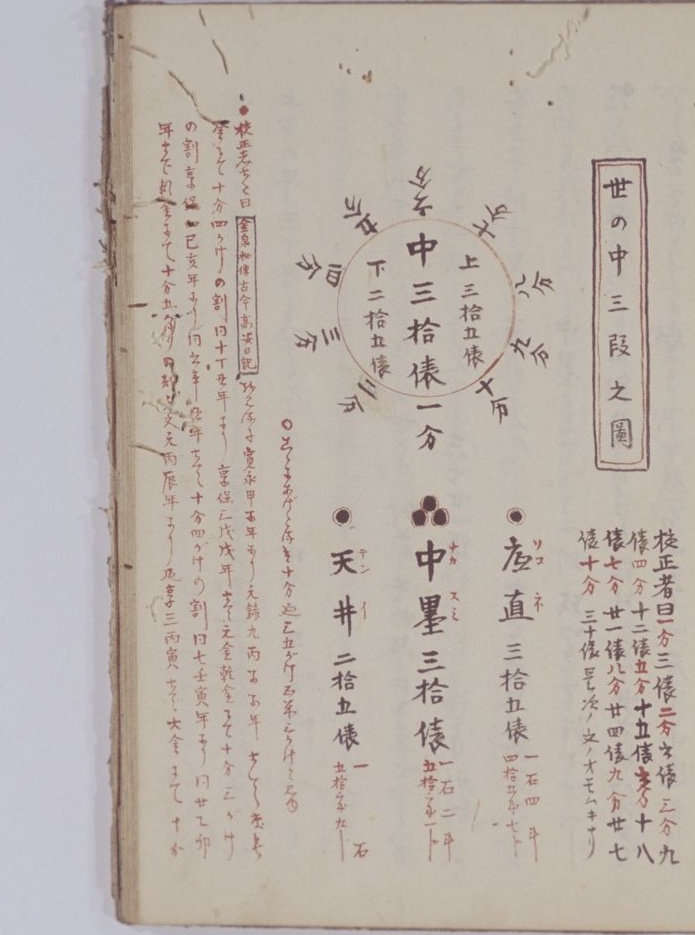
\includegraphics[width=0.55\textwidth]{diagrams/fig3_three_levels.jpg}
\caption{The Three Levels Diagram (\jp{世の中三段之圖}). The circle is
divided into Upper (\jp{上}, 35 tawara), Middle (\jp{中}, 30 tawara plus
1 bu), and Lower (\jp{下}, 25 tawara). Below: the Ceiling (\jp{天井}),
Floor (\jp{底直}), and Middle Star (\jp{中星}) reference points with their
associated price tables. \textit{Image: Kyoto University Main Library.}}
\label{fig:threelevels}
\end{figure}

\section{The Three Levels}

The rice market at any moment exists within one of three ranges:

\begin{itemize}[leftmargin=2em]
\item \textbf{Upper} (\jp{上}): approximately 35 tawara level---the ceiling
  range where selling is indicated.
\item \textbf{Middle} (\jp{中}): approximately 30 tawara, 1 bu---the
  equilibrium range where one observes and waits.
\item \textbf{Lower} (\jp{下}): approximately 25 tawara level---the floor
  range where buying is indicated.
\end{itemize}

\section{The Middle Star}

The \jt{中星}{chūboshi}, or ``Middle Star,'' is the central concept.
Across thirty years of observation, the average rice price establishes a
central equilibrium---the middle star.\tn{This is essentially a moving
average concept. The ``thirty years'' likely refers to the observational
dataset used, though the practical calculation would have used a shorter
period. The principle---trading deviations from a long-term mean---is the
foundation of modern mean-reversion strategies.} The key teaching:

\begin{itemize}[leftmargin=2em]
\item When price is \textit{at} the middle star: observe and wait.
\item When price falls to \textbf{20\% below} the middle star: begin buying.
\item When price rises to \textbf{20\% above} the middle star: begin selling.
\end{itemize}

In a year of abundant harvest, the direct price falls to the middle star or
below. One should buy at this point and hold, as in subsequent years the
price will revert.

\section{Position Calculations at the Middle Star}

The text provides exhaustive numerical examples of position-building at
each level, starting from 100 ryō and compounding through stages:

\begin{enumerate}[leftmargin=2em]
\item \textbf{First entry}: 100 ryō committed at the middle star level,
  purchasing approximately 14 tawara.
\item \textbf{Second entry}: another 100 ryō as direction confirms---total
  position now 200 ryō.
\item \textbf{Third entry}: further addition, bringing total to 300 ryō.
\item \textbf{Fourth entry}: full position established at 400 ryō, with
  compounding bringing the effective exposure to approximately 800 ryō.
\end{enumerate}

The method is then extended to 1,000-ryō and larger capital bases, always
following the same staged discipline.

% =============================================================================
% CHAPTER 9: THE SEVEN FORTUNES SECRET
% =============================================================================
\chapter{The Seven Fortunes Secret}

\begin{center}
\jp{七福即宝秘密}\\
\textit{Shichifuku Sokuhō Himitsu}
\end{center}

\vspace{1em}

This section reveals the core secret: the ``seven fortunes'' are seven
conditions that, when all are present simultaneously, indicate a
high-probability trade.

\section{The Seven Conditions}

The trader must observe:

\begin{enumerate}[leftmargin=2em]
\item The \textbf{seasonal cycle} is favorable.
\item The price is \textbf{at or below the middle star}.
\item Market \textbf{sentiment is bearish}---the crowd is selling.
\item The \textbf{harvest forecast} supports the position.
\item The \textbf{momentum} of recent days confirms a reversal.
\item One's own \textbf{capital is sufficient} to hold through adversity.
\item The \textbf{fortune-qi} (\jt{運気}{unki}) of the year aligns.
\end{enumerate}

When all seven align, one buys with full conviction through the staged
method.

\begin{maxim}
This is the ``instant treasure'' (\jp{即宝})---not that wealth comes
instantly, but that the \textit{recognition} of the opportunity must be
instant and decisive.
\end{maxim}

\section{On Patience and Money}

\begin{maxim}
There is a saying: ``The money that was thought lost returns after three
years.'' In trading, positions that seem like losses in the short term often
prove profitable in the long term---if the fundamental analysis was correct.
The error is not in the analysis but in the trader's inability to endure the
interim.
\end{maxim}

The cautious trader who holds stable reserves and trades with only a portion
of his capital will survive all storms. He who trades with his entire
fortune will eventually be ruined.

% =============================================================================
% CHAPTER 10: THE GRAND DIAGRAM
% =============================================================================
\chapter{The Grand Diagram}

\begin{center}
\jp{三割上下割之圖}\\
\textit{Sanwari Jōge Wari no Zu --- Diagram of the Three-Part Upper and Lower Division}
\end{center}

\vspace{1em}

This diagram is the visual synthesis of the entire trading system,
combining seasonal cycles, price levels, and the Yin-Yang framework into a
single reference chart.

\begin{figure}[H]
\centering
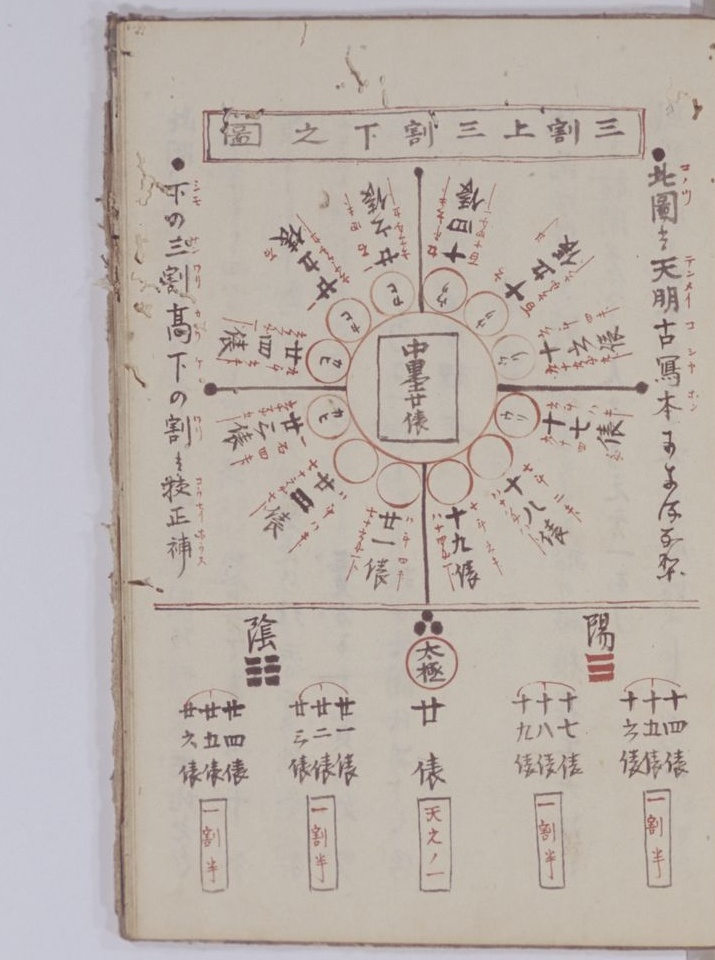
\includegraphics[width=0.7\textwidth]{diagrams/fig4_grand_chart.jpg}
\caption{The Grand Diagram (\jp{三割上下割之圖}). \textbf{Center}:
\jp{中星廿俵} (Middle Star, 20 tawara) as the equilibrium point.
Twelve positions radiate outward representing the months, each annotated
with the expected tawara level and trading action. \textbf{Bottom left}:
\jp{陰} (Yin) with the Eight Poles---selling positions at 25, 24, 22, 21
tawara levels. \textbf{Bottom right}: \jp{陽} (Yang)---buying positions at
14, 17, 18, 19 tawara. The notation \jp{天明古写本} indicates the
Tenmei-era source manuscript, annotated \jp{平の三割高下の割＝校正補}
(``Three-part division of prices, high and low---revised supplement'').
\textit{Image: Kyoto University Main Library.}}
\label{fig:grandchart}
\end{figure}

\section{How to Read the Diagram}

The diagram represents the \jp{中星圓珠秘象} (``Middle Star Round Jewel
Secret Image''). It combines the seasonal cycle with the trading method:

\begin{itemize}[leftmargin=2em]
\item The \textbf{upper half} (Yang months) represents spring and
  summer---the period of growth and rising prices.
\item The \textbf{lower half} (Yin months) represents autumn and
  winter---the period of harvest and falling prices.
\item At \textbf{each month's position}: the expected tawara level, the
  indicated trading action (buy, sell, or hold), and the relationship to
  the middle star.
\end{itemize}

In the four directions---representing the four seasons---one combines the
seasonal tendency with the harvest forecast. When buying in spring, confirm
the middle star level, then enter at the 10\% level.

% =============================================================================
% CHAPTER 11: READING STRONG AND WEAK QI
% =============================================================================
\chapter{Reading Strong and Weak Qi}

\section{The Beginning of Strong Qi}

\begin{maxim}
When strong qi first emerges, the signs are these: a ten-percent rise from
the bottom; people are still bearish; news is still negative; yet the price
has stopped falling and begins to creep upward.\\[0.5em]
This is the critical moment to begin buying.
\end{maxim}

Just as strong qi begins silently amid pessimism, weak qi
(\jt{弱気}{yowaki}) begins silently amid optimism. The master trader reads
both transitions.

\section{The Beginning of Weak Qi}

The counterpart to strong qi:

\begin{maxim}
A small decline from a sustained high. People are still bullish. Good news
continues. Yet the price stops rising and begins to soften.\\[0.5em]
This is when selling should begin.
\end{maxim}

The symmetry is exact---the same pattern, inverted.

\section{The Great First Decline}

When a major correction begins:

\begin{maxim}
The first drop is sharp and frightening. Panic selling follows. But the
first major drop is rarely the final bottom.\\[0.5em]
After the panic subsides, a temporary recovery occurs. Then the slower,
grinding decline continues to the true bottom.
\end{maxim}

This pattern---sharp drop, bounce, slow grind---repeats across all markets
and all eras.\tn{This three-phase decline pattern is remarkably similar to
Dow Theory's description of bear market stages, formulated by Charles Dow
nearly fifty years later, and to modern descriptions of market crash
anatomy. The Edo-period rice traders identified the same dynamics through
pure observation.} Patience is required to wait for the true bottom rather
than buying the first panic.

\section{Wind and Rain}

Wind and rain are both literal and metaphorical:

\begin{maxim}
When a storm comes and the ship is at sea, one cannot change the wind. But
one can adjust the sails.\\[0.5em]
Similarly, when market conditions shift suddenly, one cannot change the
conditions, but one can adjust the position.
\end{maxim}

The four seasons each bring their own storms. The trader who anticipates
them is rarely caught off guard.

% =============================================================================
% CHAPTER 12: REGIONAL MARKETS AND FINAL TEACHINGS
% =============================================================================
\chapter{Regional Markets and Final Teachings}

\section{The Geography of Information}

Osaka's D\=ojima exchange is the central rice market; all other regional
prices reference it. The information from Osaka flows outward to the
provinces, and the gap between Osaka and provincial prices creates trading
opportunities.

\begin{maxim}
The trader in the provinces who knows the Osaka price has an advantage over
one who knows only local prices.
\end{maxim}

Eastern provinces and western provinces have different harvest cycles. When
eastern harvests are poor but western harvests are good, the price in Osaka
reflects the average. A trader who can read the signs in the fields before
the market knows has the greatest advantage.

\section{The Essence of the Teaching}

In all the world's markets, the rice market is the foundation. What has
been written in this record is the accumulated observation of
generations---the secret teachings of the house, refined and corrected.

\begin{maxim}
The market is not a place of chance but of pattern. Those who study the
patterns---of seasons, of cycles, of human sentiment---can trade with the
odds in their favor.\\[0.5em]
But even the most learned trader will sometimes be wrong, and the method of
staged entry and proportional trading exists precisely for this reason: to
survive being wrong while maximizing the benefit of being right.
\end{maxim}

\section{The Four Virtues, Restated}

One should approach the market with the same virtues that govern all of life:

\begin{itemize}[leftmargin=2em]
\item \jt{仁}{Jin} --- \textbf{Benevolence}: patience and compassion for
  one's own errors.
\item \jt{智}{Chi} --- \textbf{Wisdom}: study and observation before action.
\item \jt{勇}{Yū} --- \textbf{Courage}: acting decisively when the signs
  align.
\item \jt{節}{Setsu} --- \textbf{Discipline}: following the method even
  when emotions urge otherwise.
\end{itemize}

\begin{maxim}
The trader who embodies all four virtues will prosper across generations.\\
The trader who relies on any one alone will eventually fail.\\[0.5em]
This record should not be shared carelessly. It represents a lifetime---indeed,
many lifetimes---of observation, and its value lies not merely in the rules
but in the \textbf{understanding} behind them.\\[0.5em]
A rule without understanding is dangerous;\\
understanding without discipline is useless.\\[0.5em]
To the reader who has studied this record thoroughly:\\
may you trade with wisdom and prosper.
\end{maxim}

\begin{flushright}
\jp{鳴川猛之助}\\
\textit{Narukawa Takenosuke}\\
\textit{Editor and Corrector}
\end{flushright}

% =============================================================================
% GLOSSARY
% =============================================================================
\chapter*{Glossary of Key Terms}
\addcontentsline{toc}{chapter}{Glossary of Key Terms}
\markboth{Glossary of Key Terms}{}

\begin{description}[style=nextline, leftmargin=2em, font=\normalfont\bfseries]

\item[\jp{逢来} (\textit{airai})]
Adverse conditions. A period of generally falling rice prices and poor
market conditions, typically lasting roughly three years within a
twelve-to-thirteen-year cycle.

\item[\jp{中星} (\textit{chūboshi})]
Middle Star. The long-term average rice price level that serves as the
central reference point for all trading decisions. Analogous to a moving
average in modern technical analysis.

\item[\jp{堂島} (\textit{Dōjima})]
The D\=ojima Rice Exchange in Osaka, the central marketplace for rice
futures trading during the Edo period.

\item[\jp{帳合米} (\textit{chōaimai})]
``Book rice.'' Forward contracts or futures on rice traded at the D\=ojima
exchange, as opposed to physical rice.

\item[\jp{人気} (\textit{jinki})]
``People-qi.'' Market sentiment; the collective mood of traders.

\item[\jp{順来} (\textit{junrai})]
Favorable conditions. A period of generally rising rice prices, typically
lasting roughly ten years.

\item[\jp{古米} (\textit{komai})]
Old rice. Rice from previous harvests, traded as a distinct commodity.

\item[\jp{新米} (\textit{shinmai})]
New rice. Freshly harvested rice.

\item[\jp{太極} (\textit{taikyoku})]
Supreme Ultimate. The Neo-Confucian concept of the undifferentiated unity
from which Yin and Yang emerge; here used to represent market equilibrium.

\item[\jp{天井} (\textit{tenjō})]
Ceiling. The top of the price range; the point beyond which prices are
unlikely to rise further.

\item[\jp{底} (\textit{soko})]
Bottom or floor. The lowest point of the price range.

\item[\jp{強気} (\textit{tsuyoki})]
Strong qi; bullish sentiment or upward momentum.

\item[\jp{運気} (\textit{unki})]
Fortune-qi. The prevailing momentum or fortune of a given period, combining
seasonal, cyclical, and weather-related factors.

\item[\jp{弱気} (\textit{yowaki})]
Weak qi; bearish sentiment or downward momentum.

\item[\jp{俵} (\textit{tawara} / \textit{hyō})]
A bale of rice; the standard unit of measure for rice trading. Also used
as a unit of price quotation.

\item[\jp{両} (\textit{ryō})]
The gold coin unit of the Edo period; the standard unit of capital and
accounting.

\end{description}

\vfill

\begin{center}
\rule{2in}{0.4pt}\\[1em]
{\small\itshape End of the Complete Volume}\\[0.3em]
{\small \jp{全} --- \textit{Zen}}
\end{center}

\end{document}
